\documentclass[dvipsnames,a4paper,11pt]{article}

\usepackage[utf8]{inputenc}
\usepackage[T1]{fontenc}
\usepackage{a4wide}
\usepackage{amsmath}
\usepackage{todonotes}
\usepackage{xcolor}
\usepackage{amsthm}
\usepackage{amssymb}
\usepackage{accents}


\newtheorem{thm}{Theorem}
\newtheorem{prop}{Propery}

\theoremstyle{definition}
\newtheorem{defn}{Definition}

\theoremstyle{remark}
\newtheorem{rmq}{Remark}

\theoremstyle{remark}
\newtheorem{ex}{Example}

\newcommand{\tiph}[1]{\todo[inline,color=Orchid]{#1}}
\newcommand{\pimprenelle}[1]{\todo[inline, color=ForestGreen]{#1}}
\newcommand{\jeffin}[1]{\todo[inline, color=BrickRed]{#1}}
\newcommand{\jeff}[1]{\todo[color=BrickRed]{#1}}


\title{Multiplex stream graphs}
\author{Pimprenelle Parmentier, Tiphaine Viard, \ldots}

\begin{document}
    \maketitle

    \section{Multilayer stream graphs}

	\subsection{Preliminaries}
	
	\pimprenelle{ajout des définitions préliminaires. J'ai essayé d'être concise, tout en renvoyant à nos deux papiers de référence }	
	
	To understand well the notion of multilayer stream graph, it is important to know the multilayer graphs and the stream graphs. We will give a short definition of each object.
	
	\begin{defn}[Graph]
	    A graph $G=(V,E)$ is a set of "vertices" V, and of "edges" E. An edge represents an interaction between two vertices.
	\end{defn}
	
	\begin{defn} [Multilayer graph]
    A multilayer graph \cite{mlkiv} is a 4-element set $M=(V_M,E_M,V,L)$. V is a set of nodes which can belong to different layers. The structure of the layers is modeled by $L=(L_1,\dots L_n)$. Each $L_i$ is a set of "elementary layers". An elementary layer is an n-uplet of ${\bf L} = L_1\times L_2 \times \dots L_n$. A node in a layer is called "node-layer", the corresponding set is $V_M$. Then $E_M$ is the set of edges between node-layers.
	\end{defn}
	
	The multilayer graphs have been created to describe graphs in which d nodes  can have different properties (represented by the layers) and diff
	
	\begin{defn}[Stream graph]
	   \cite{stream} Let $T$ be a time interval, and $V$ a set of nodes. $W$ is a set of elements $(t,v), t\in T$ and represents the apparition of nodes during the time. $E$ is a set of triplets $(t,u,v)$ such as $(t,u)$ and $(t,v)$ are in $W$, and represents the links as function of time. A {\em stream graph} is the quadruplet $S=(T,W,V,E)$.
	    
	    We call $T_u$ the set of time $t$ such as $(t,u)$ is in W, and $T_{uv}$ contains all the $t$ such as $(t,u,v)$ are in $E$.
	\end{defn}
	
    Through this paper, each time we will define a new "measure" for multilayer stream graphs, we will make the link with the corresponding notion in the multilayer graphs and in the stream graphs, when it is relevant. This will demonstrate that multilayer stream graphs are a generalisation of the two concepts.
	
	
	\subsection{Definition}	
	\begin{defn}[Multilayer stream graph]
    We define a multilayer stream graph as a tuple $S_M = (T,T_M,V,W_M,E_M,{\cal L})$, such that $T$ and $V$ are, respectively, a time interval and a set of nodes, just like for stream graphs \cite{stream}.
    
    As for multilayer graphs \cite{mlkiv}, ${\cal L}$ is a set of $d$ {\em aspects}; ${\cal L} = \{L_i\}_{i=1}^d$, and an element $\alpha_i$ of $L_i$ is named {\em elementary layer}. An element of $L=L_1\times \dots \times L_d$ is named {\em layer}.

	$T_M$ is a set of intervals of $T$ so for that each layer $\alpha$, $T_{\alpha}$ is the interval at which the layer exists. For each $t$ in $T$, $\exists \alpha \in L | t \in T_{\alpha}$. At each time of $T$, at least one layer of $L$ exists.

	$W_M \subseteq T\times V \times (L_1 \times \dots \times L_d)$ represents the existing points on layers with respect to time. For each element $(t,u,\alpha)$ of $W_M$, $t$ must be in the interval of existence of $\alpha$.

   $E_M \subseteq T\times V_M \otimes V_M$ are the links appearing with respect to time,  $V_M = \{ (u,\alpha), u\in V, \alpha \in L\}$. The elements of $V_M$ are named {\em node-layer}. A link cannot appear outside the time of existence of the two node-layers.

    Notice that just like in multiplex networks, nodes in time ({\em i.e.}, elements of $W_M$) can be present in an arbitrary number of layers.
	\end{defn}
	
   	\pimprenelle{La représentation de la présence ou non des couches en fonction du temps par $T_M$ est un choix, que nous préférons pour le moment à celle $M_M$ des couples $(t,\alpha)$}
   	
   	\pimprenelle{Ajout des contraintes sur les temps d'existence des node-layers et des links}

	\subsection{2 examples}
	\begin{ex}[Research world]\label{exresearch}
	We consider a set of researchers.
	
	These people can work in one or more universities and/or companies, in one or more departments. They can work together on different ways : they can collaborate on a paper, supervise or being supervised. And their work on different subjects, linked together thanks to keywords.


	In this multilayer stream graph, the {\bf nodes V} are the researchers. The {\bf aspects L} are the university/companies , the departments, the subjects, the type of status of interaction (supervisor/ supervised / collaborator). {\bf Links} appear during an interaction between two researchers, for example if they work together on the same paper. The layers, researchers, and collaborations vary with time, this gives us the stream aspect.
	
	\end{ex}
	
	\begin{figure}[h]
    	\centering
    	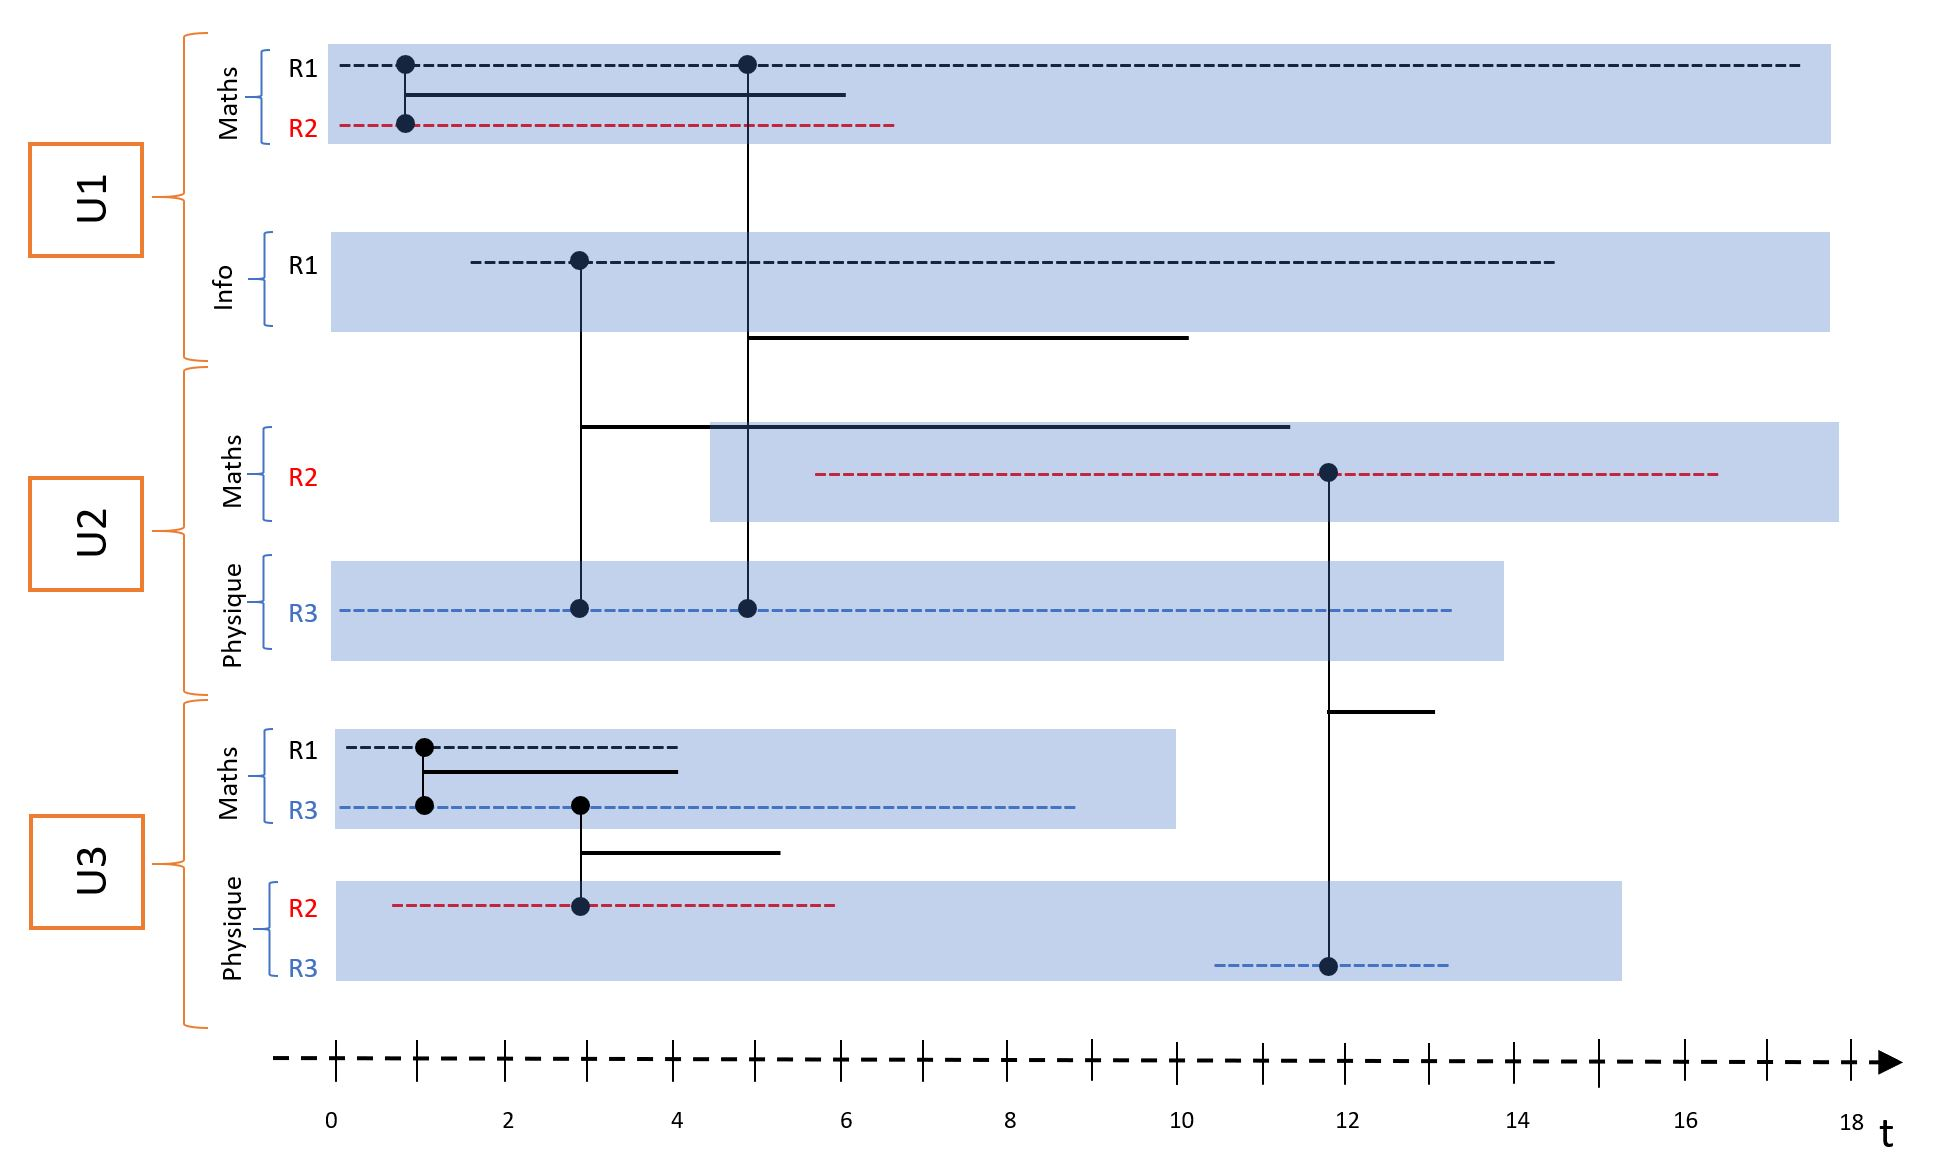
\includegraphics[width=15cm]{schemas/chercheurs.jpg}
    	\caption{An simplified scheme of a multiplex stream graph for example \ref{exresearch}.\newline
    	$T=[0,10], V=(R_1,R_2,R_3), L = [[U1,U2,U3],[Math,Info,Physics]]$\newline
    	$T_M=([0,10]\times\{[U1,Maths],[U1,Info]\})\cup([4,10]\times\{[U2,Maths]\})\cup\dots$\newline
    	$W_M=[0,10]\times \{(R1,[U1,Maths])\}\cup ([0,7]\times \{(R2,[u1,Math])\}\cup\dots $\newline
    	$E_M = [0,6]\times[(R1,[U1,Maths]),(R2,[U1,Maths])] \cup [1,4]\times [(R1,[U3,Maths]),(R3,[U3,Maths])] \cup \dots$}
    	\label{fig:chercheurs}
	\end{figure}
	
	
	\pimprenelle{cet exemple risque d'être retiré au profil de celui des lignes d'avion (puisqu'on a le dataset). Pas facile du tout de trouver un dataset d'espèces animales, il faudrait qu'ils portent des puces capables de nous dire quel type d'interaction ils ont eues, à quel moment ils tombent malades... ou peut être générer un graphe aléatoirement et vraisemblable ?}

	\begin{ex}[Epidemics between species]
		We consider an set of individuals from different species, and a disease. This disease could be transmitted through different types of interaction : by blood, by  by respiratory tracts, digestive tracks, etc.
		
		We can model this system with a multilayer stream graphs. The nodes would be the individuals, and the aspect their characteristics : their species, the type of possible interaction (predator, parasite), the state of the individual (sane, infected, contagious, dead, healed ... ). The links appear when there is an interaction between two individuals, the type of the link depends on the two layers of the nodes. This system is time-dependant, and we can draw the corresponding stream.
	
		The question here could be : when and where do we have to act (cut some connection / remove some node-layer) to stop the spreading of the disease as soon as possible ?
	\end{ex}

	
	\begin{rmq}
		We notice that it is easy to make the multilayer as complex as we want. Three rules seem to be important to have a pertinent use of multiplex-stream graph :
		\begin{itemize}
			\item a set of nodes which could have various properties which can be "melted"
			\item different ways to interact between the nodes in function of their properties
			\item a time-dependency
		\end{itemize}
	\end{rmq}
	
	\newpage
	
   	\section{Substreams and operations over substreams}

    From this definition, let us define common streams of interest. Depending on what we need, we can extract the stream of one layer, or the stream of interactions between two layers.
	
	We can begin to "classify" edges according to the nature of their nodes : 
	
	\begin{defn}[Coupling, intra-layer and inter-layer edges]

   	The {\em coupling edges} are $E_C=\{(t,u,\alpha,v,\beta)\in E_M | u=v\}$.

    The {\em intra-layer edges} are $E_I = \{(t,u,\alpha,v,\beta) \in E_M | \alpha = \beta \}$

    The {\em inter-layer edges} are $\bar{E_I} = E_M\backslash E_I$.
    
	(See fig.\ref{exIntraInter} for a visual representation.)
	
	\end{defn}	
	
	\begin{figure}[h]
		\centering
		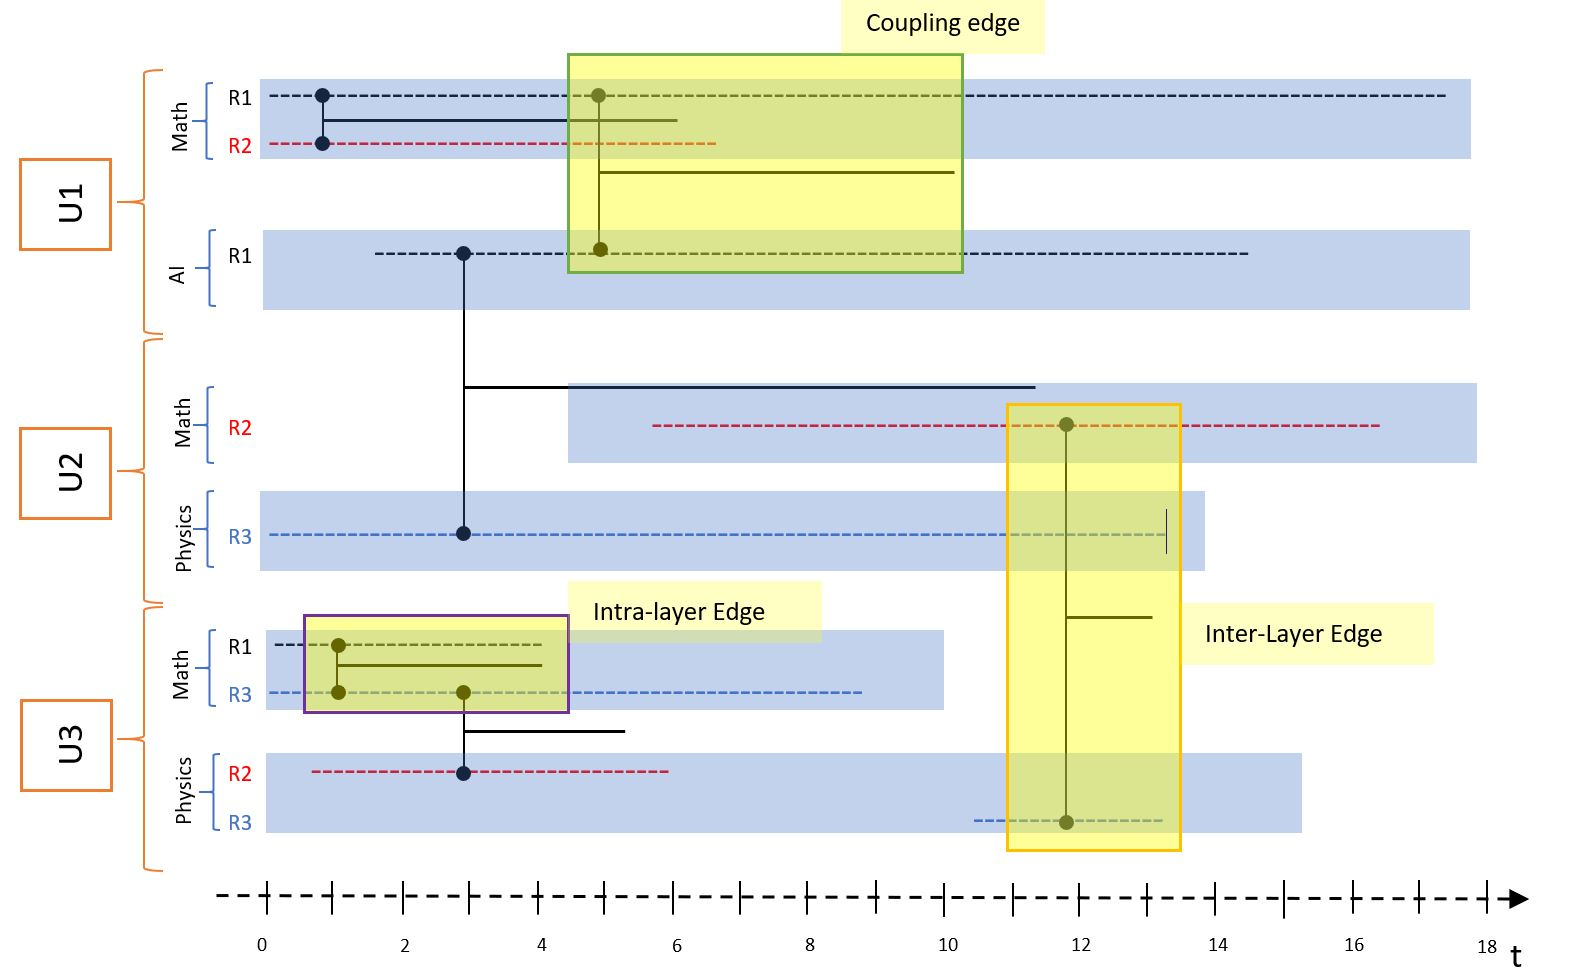
\includegraphics[width=\textwidth]{schemas/edgesCat.jpg}
		\caption{Illustration with our example of coupling edges, intra-layer edges and inter-layer edges}
		\label{exIntraInter}
	\end{figure}
	
	In the multilayer graph theory, the multiplex graphs have some specific properties and some tools have been created to study their properties. We define here the multiplex stream graph.
	
	\begin{defn}[Multiplex stream graph]	
	A {\em multiplex stream graph (MpSG)} is a graph in which edges are either coupling edges or intra-layer edges.
	\end{defn}
	
	
	 
	\begin{defn}[Intra-layer stream graph]
	For any layer $\alpha \in L_1 \times \dots \times L_d$, the {\em intra-layer} stream graph $S^{\alpha}$ is the stream $S^{\alpha}=(T^{\alpha},V^{\alpha},W^{\alpha},E^{\alpha})$ such that $T^{\alpha} = T_{\alpha} \in T_M$ is the interval of existence of $\alpha$. $V^{\alpha}$ is the set of node-layers on the layer $\alpha$ and $W^{\alpha}$ are their time of appearance on this layer. $E^{\alpha}$ is the subset of $E_M$ containing only the links between the nodes-layers of $\alpha$.
	\end{defn}
	
	
	\begin{defn}[Inter-layer stream graph]	
	For any two layers $\alpha, \beta \in L_1\times \dots\times L_d$, the {\em inter-layer} stream graph is the stream $S^{(\alpha,\beta)} = (T, V^{\alpha,\beta},W^{\alpha,\beta},E^{\alpha,\beta})$ such that : $T^{\alpha,\beta}=T^{\alpha}\cap T^{\beta}$ is the interval of time in which $\alpha$ and $\beta$ appear simultaneously. $V^{\alpha,\beta}$ are all the node-layers of the multiplex stream graphs which are in the layers $\alpha$ and $\beta$, $W^{\alpha,\beta}$ describes theirs intervals of appearance. Then, $E^{\alpha,\beta}$ are the undirected links between nodes-layers of $\alpha$ and $\beta$ with their times of occurrence.
	\end{defn}
	
	Notice that for any layer $\alpha$, $S^{(\alpha)}$ is equivalent to $S^{(\alpha,\alpha)}$.

	\section{Intersection and union}
	
	After extracting some layers or inter-layer graphs, we might want to study a few layers at the same time, or to study an intersection.
	
	We built then the tools adapted.
	
	\begin{defn}[Intersection of two substreams]
	The {\em intersection} of two substreams $S_1$ and $S_2$ is defined as follows :
	\[
		S' = S_1 \cap S_2 = (T_1\cap T_2, V_1 \cap V_2, W_1 \cap W_2, E_1\cap E_2)
	\]
	\end{defn}
	
	Notice that this intersection is a stream graph too.

	\begin{defn}[Union of two substreams]
	The {\em union} of two substreams $S_1$ and $S_2$ is defined as follows :
	\[
		S' = S_1 \cup S_2 = (T', V_1 \cup V_2, W_1 \cup W_2, E' \})
	\]
	As $T'$ should be an interval, we take the shortest interval containing $T_1$ and $T_2$.
	\[
		T' = [\min(T_1,T_2),\max(T_1,T_2)]
	\]
	\[
		E' = E_1 \cup E_2 
	\]
	We note that the union stream graphs contains at least two connected components with this definition.
	
	Notice that the union of two sub stream graphs gives a stream graph.
	\end{defn}
	
	
	\begin{defn}[Underlying stream]
		The {\em underlying stream } $S_U(S_M)$ of $S_M$ is $(T,V_M,W_M,E_M)$. Its is the stream graph in which the nodes are the node-layers. It could be shared into clusters corresponding to the different layers. This definition is a generalisation to the one defined on \cite{mlkiv} for simple multilayer graphs.
	\end{defn}
	
	\begin{defn}[Aggregated stream]
		
		The {\em aggregated stream} $S_A(S_M)$ has the same $T$ as $S_M$. Its nodes are the nodes of $S_M$ and a link exists between two nodes if and only a link exist between two correspondent node-layers.	This definition is a generalisation to the one defined on \cite{mldd} for simple multilayer graphs.
	
	\end{defn}
	
	We can now demonstrate that the underlying stream graph is the union of all the intra and inter layer stream graphs.
	
	\begin{prop}
		\[
			\bigcup_{(\alpha,\beta) \in L^2} S^{(\alpha,\beta)} = S_U(M_S)
		\]
	\end{prop}
	\begin{proof}
	We call $S=\bigcup_{(\alpha,\beta) \in L^2} S^{(\alpha,\beta)}=(T^{*},V^{*},W^{*},E^{*})$ and we want to show that $S=S_U(M_S)=S_U(M) = (T_U,V_U,W_U,E_U)$.
	
	$T=T_U$ by definition of $S_U$. By construction of multilayer stream graphs, at each $t\in T$, at least one layer $\alpha$ is existing. Then as $T* = [\min_{\alpha \in L} (T^{\alpha}),max_{\alpha \in L} (T^{\alpha})]$, $t$ is included in $T*$. Each $T^{\alpha}$ is included in $T$, so $T^* \subseteq T$, which leads us to $T^*=T_U=T$.
	
	$V_M = V_U$ by definition of $V_U$.$V^{*}=\bigcup_{(\alpha,\beta) \in L^2} V^{\alpha,\beta} \subseteq V_M$. All the nodes of all the layers are included in $\bigcup_{(\alpha) \in L^2} V^{\alpha,\alpha} \subseteq V^{*}$, so we obtain the equality $V_M=V_U=V^*$.
	With the same argument we find that $W_M=W_U=W^*$.
	
	$E_U=E_M$ and $E^{*}=\bigcup_{\alpha,\beta \in L^2}(E^{\alpha,\beta})$ by definition. So as $E^{\alpha,\beta}$ is a subset of $E_M$ for every couple of layers $\alpha,\beta$, $E^{*} \subset E_M$. We notice too that for every $e =(t,u,\alpha,v,\beta) \in E_M$, $e$ belongs to $E^{\alpha,\beta}$. So $\mathbf{E_M=E^{*}}$.
					
	\end{proof}
	
	
	\section{Projections on the time}
	
	We can then decide to aggregate informations during the time or to select informations at a certain time.
	
	We can first decide to "take a picture" of the graph at a precise time t :
	\begin{defn}[Multilayer graph at time t]
   	The {\em multilayer graph at time t} $M_t$ is $M_t = (V_{M,t}, E_{M,t},V,{\cal L})$ with $V_{M,t}$ and $E_{M,t}$ containing all the node-layers and links appearing at $t$.
   	$$ V_{M,t} = \{ (u,\alpha) | (t,u,\alpha) \in W_M\} $$
   	$$ E_{M,t} = \{(u,\alpha,v,\beta) | (t,u,\alpha,v,\beta) \in E_M\}$$

   \end{defn}

	\begin{figure}[h]
		\begin{minipage}{0.49\linewidth}
			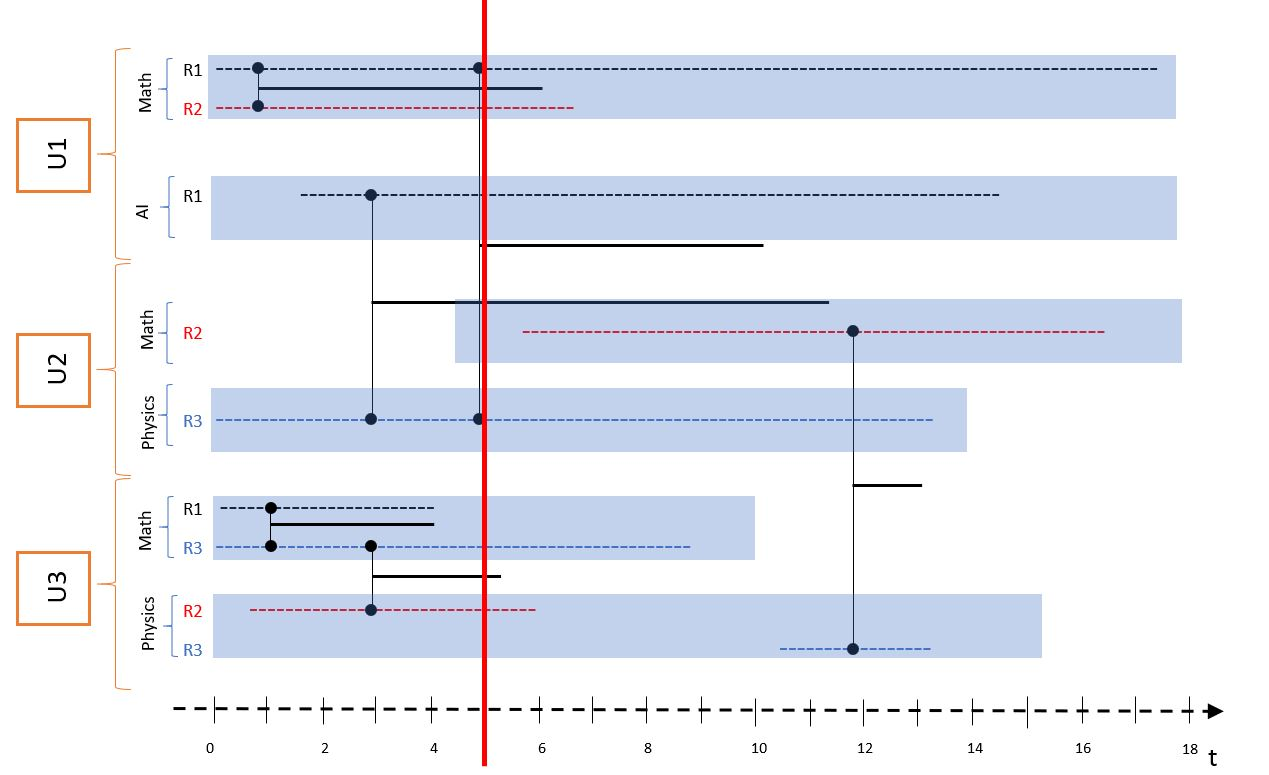
\includegraphics[width=\textwidth]{schemas/pauset.jpg}
		\end{minipage}
		\begin{minipage}{0.49\linewidth}
			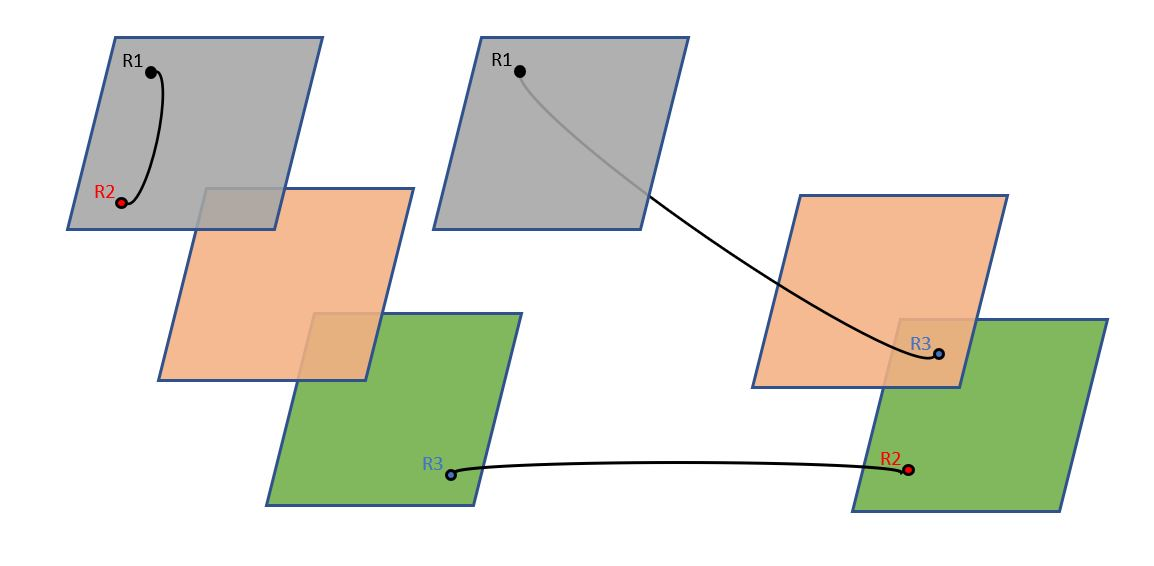
\includegraphics[width=\textwidth]{schemas/pausetproj.jpg}
		\end{minipage}
		\caption{Our multilayer example at time $t=5$}
	\end{figure}

    
    The {\em multilayer graph induced} $M_I(S_M) = (V_{M,I}, E_{M,I}, V,L)$ of $S_M$ is the multilayer graph which gather all the layers, node-layers and links which appear during $T$.
    \begin{align*}
    	V_{M,I} = \bigcup_{t\in T} V_{M,t}\\
    	E_{M,I} = \bigcup_{t\in T} E_{M,t}\\
    \end{align*}
    
	
	We notice that many graphs are actually extracted from multilayer stream graphs, with the different operations we presented.	
	
	For example, the page-rank algorithm uses the aggregated and induced graph of the multilayer stream graph looking like the one of our example. The temporal and multilayer informations have been "lost" in this operation but we understand well that they existed at the beginning.
	
	
	\section{Number of nodes, number of layers}
	
	We might want then to quantify the presence and the number of interactions in a multilayer stream graph. We will propose a few measures which take into account the multilayer and the stream aspect.
	
	The {\em number of nodes in a graph} $G=(V,E)$ is $|V|$ and the number of edges is $|E|$.
	
	The {\em number of nodes in a stream graph} $S=(T,V,W,E)$ has been defined in \cite{stream} as $\hat{N}^T_n=\frac{|W|}{|T|}=\sum_{v\in V} n_v$. $n_v$ is called the {\em contribution of v} and is equal to $\hat{N}^T_v=\frac{|T_v|}{|T|}$. Note that this notion is different to the {\em number of nodes in the graph} $|V|$.
	\newline
	
	In multilayer graphs, such similar notion hasn't been explicitly defined as far as we know.
	Rather than just counting the nodes or the node layers, we define the {\em average number of nodes by layer} as :
	\begin{align*}
		\hat{N}_n^L(M_l) = \frac{\text{number of node-layers}}{\text{number of layers}}=\frac{|V_M|}{|L|}
	\end{align*}	    
	Notice that if there is only one layer, we find the classical number of nodes, which means that this definition is a generalisation of the number of nodes for multilayer graphs.
		
	
	\begin{defn}[Contribution of layer]
	We define too the {\em contribution} of one layer as follows : $n_\alpha = \frac{|T_{\alpha}|}{|T|}$. The {\em number of layers in a multilayer stream graph} is then the sum of their contributions. $\hat{N}^T_l = \sum_{\alpha \in L}\frac{ |T_{\alpha}|}{|T|}$
    \end{defn}
	
	\begin{defn}[Contribution and quantity of node-layers]
	The {\em contribution of one node-layer} in the multilayer stream graph is $n_{v,\alpha} = \frac{|T_{v,\alpha}|}{|T|}$. The {\em number of node-layers} is the sum of the contributions $\hat{N}^{T}_{nl}(M) = \underset{(u,\alpha)\in V_M}{\sum} n_{(u,\alpha)} = \frac{|W_M|}{|T|}$.
    \end{defn}
	
	Notice that if we have only one layer, we find the number of node-layers which is the number of nodes. If we take the underlying stream of the multilayer stream graph, we find too the same number of node-layers.

    
    We decide then to define the \textbf{number of nodes in a multilayer stream graphs} as follows : 
    
    \begin{defn}[Contribution and number of nodes]
    The {\em contribution} of a node describes the rate of appearance of the node on the different layers : $n_v = \frac{\sum_{\alpha \in L}|T_{v,\alpha}|}{\sum_{\alpha \in L} |T_{\alpha}|}$.
    
    The {\em quantity of nodes} is then the sum of the contribution of the nodes : 
    \begin{align}
    \hat{N}^{L,T}_n(M) = \sum_{v\in V} n_v= \sum_{v\in V} \frac{\sum_{\alpha \in L}|T_{v,\alpha}|}{\sum_{\alpha \in L} |T_{\alpha}|} 
    \label{numberNodes}
	\end{align}     
	
	\end{defn}
	
	This definition is coherent with the notions in multilayers and stream graphs : if the node appears in all the layers all the time, we find $n_v = 1$ like in multilayers. If all the times of existence are all equals, whe find $n_v=\frac{\text{number of node-layers of node v}\times |T|}{\text{number of layers}\times |T|}$. This definition is then a good generalisation of the two notions.
	
	\section{Uniformity}
	
	In stream graph the {\em uniformity between a pair of nodes} $u$ and $v$ is the ratio $\Cup (u,v) = \frac{|T_u\cap T_v|}{|T_u \cup T_v|}$. It measures how much two nodes can be linked together.
	
	
	The {\em uniformity } of two nodes-layers $(u,\alpha)$ and $(v,\beta)$ measures the rate of overlap presence of two node-layers, their "theoretical" ability to be linked together.
	\begin{align*}
		\Cup((u,\alpha),(v,\beta))=\mathbb{P}( t \in T_{u,\alpha} \cap T_{v,\beta} | t \in T_{u,\alpha} \cup T_{u,\beta}) \\
		= \frac{|T_{u,\alpha}\cap T_{u,\beta}|}{|T_{u,\alpha}\cup T_{u,\beta}|}
	\end{align*}

	The {\em overlap presence} of two layers $\alpha$ and $\beta$ is defined on the same pattern :
	\begin{align*}
		\cup(\alpha,\beta) = \frac{|T_{\alpha}\cap T_{\beta}|}{|T_{\alpha}\cup T_{\beta}|}
	\end{align*}

    The {\em node-layer uniformity} measures the rate of simultaneous presences of node-layers in the multilayer-stream graph :
    \[
    	\Cup(M) = \frac{\sum_{(u,\alpha),(v,\beta) \ V_M \otimes V_M}{|T_{(u,\alpha)} \cap T_{(v,\beta)}|}}{\sum_{(u,\alpha),(v,\beta) \ V_M \otimes V_M}{|T_{(u,\alpha)}\cup T_{(v,\beta)}|}}
    \]
	
	But we could nuance this definition by taking into account special multilayer stream graphs, in which only some of the edges are allowed. For instance, in a multiplex stream graph, the only inter-layer edges allowed are the edges between the same node. So the {\em uniformity of the multiplex stream graph} will be :
	\[
    	\Cup(M) = \frac{1}{|L|}\sum_{\alpha \in L} \frac{\sum_{(u,\alpha),(v,\alpha) \ V_M \otimes V_M}{|T_{(u,\alpha)} \cap T_{(v,\alpha)}|}}{\sum_{(u,\alpha),(v,\alpha) \ V_M \otimes V_M}{|T_{(u,\alpha)}\cup T_{(v,\alpha)}|}}
    \]
	
	
	
	\begin{rmq}
		Note that this concept can be used for sub-stream graphs of any type.
	\end{rmq}

	When $\Cup=1$, we say that the multilayer stream graph is uniform.



    \section{Density}
    
    After measuring how much a graph "can be connected" with the uniformity, we will measure how actually it is connected compared to how it could be.
    
	In classical graphs (unweighed and non directional), the {\em density} $d(G)$ measures how much the vertexes are connected.
		\[
			d(G) = \frac{|E|}{|V\otimes V|} = \frac{2\times |E|}{|V|(|V|-1)}
		\]
	In stream graphs, the density measures too the "rate of connectivity", or the probability that, at a randow time when two point exist, they are connected.

		\begin{align*}
			\delta_s(G) = & \mathbb{P}((t,u,v)\in E| (t,u),(t,v) \in W) \\
			 =  & \frac{\sum_{uv \in V \otimes V}{|T_{uv}|}}{\sum_{uv \in V\otimes V}{|T_u\cap T_v|}}= \frac{\int_{t\in T}{|E_t|dt}}{\int_{t\in T}{|V_t\otimes V_t|dt}}
		\end{align*}

	We can then define the density of the multilayer graph. Notice first that the density measures the rate of connectivity, and so depending to the type of system we study, the definition can change. If some connections are forbidden, we will ignore them in the density. We name $C \in V_M\times V_M$ the set of possible connections in the mutlilayer. If some connections are automatics (like the ones between the same node in different layers), we don't take it into account too.
	\[
		\delta_M (M) = \frac{|E_M|}{|\{\text{"possible connections"}\}|}
	\]

	The generalisation to multilayer stream graphs is then natural.
	\[
		\delta_M (M) = \frac{\int_{t\in T}|E_M,t|}{\int_{t\in T}|C|} = \frac{\sum_{(u,\alpha)(v,\beta) \in V_M \otimes V_M}|T_{(u,\alpha)(v,\beta)}|}{\sum_{(u,\alpha)(v,\beta) \in C}|T_{(u,\alpha)}\cap T_{(v,\beta)}|}
	\]

	For example, in a multiplex stream graph, $C=\{(t,u,\alpha),(t,v,\beta))| t\in T_{u,\alpha} \cap T_{u,\beta}, u=v \text{or} \alpha = \beta)\}$ :

	\[
		\delta_M (M) = 
		\frac{|E_M|}{|C|}= 
		\frac{\sum_{(u,\alpha)(v,\beta) \in (V_M \otimes V_M)} |T_{(u,\alpha)(v,\beta)}|}
		{\underbrace{(\sum_{\alpha \in L}\sum_{(u,v) \in V\otimes V}|T_{u,\alpha} \cap T_{v,\alpha}|)}_{\text{intra-layer possible nodes}}+\underbrace{( \sum_{u \in V } \sum_{(\alpha,\beta) \in L \otimes L}|T_{u,\alpha}\cap T_{u,\beta}|)}_{\text{inter-layer possible nodes}}}
	\]

		\section{Neighbours and degrees}
	
		In classic graphs, the degree of a node is the number of its neighbours. The neighbours are the nodes for which a link exists between the first node and the neighbour.
		
		\subsection{Neighbours and degree in multilayer graphs}
		
		In the multilayer graphs, it is a more tricky question to know who are the neighbours of a node. In many multiplexes, the nodes-layers corresponding to the same node are linked together with an "invisible" connection. The main question should be of course : "what do we want to measure ?" We will give a few examples of different situations and the definition of the degree associated.
		
		I the case of a transportation multiplex, our nodes are some cities, the layers are different means of transportation. If we want to know how many cities you can reach from Tokyo without correspondence, we will calculate the degree of Tokyo in the aggregated graph.
		
		But we might want to highlight the fact that it is not equivalent to have one or many different links in different layers between two nodes. For example, two cities will be better connected if we can take the train or the plane to travel between them.  We then can take the sub-multilayer graph of the neighbours of all the node-layers labelled Paris, and compute the number of nodes as defined in \ref{numberNodes}. 
		
		The definition in \cite{BERL} allows us to capture the dimensional side of neighbours in multiplexes, we generalize it to multilayer graphs.
		
		\begin{defn}[The function neighbouring in multilayer graphs]
		 Let $v \in V$ be a node and $D \in L$ a set of couples of layers of $M=(V_M,E_M,V,L)$. 
		 
		 $Neighbours(v,D): \left\{ 
		 	\begin{array}{lcl}
		 		V\times {\cal P}(L \times L)& \rightarrow & \mathbb{N}\\
		 		(v,D) & \rightarrow & |\left\{u \in V | \exists (u,\alpha,v,\beta) \in E, (\alpha,\beta) \in D\right\}|
		 	\end{array}
		 	\right.$
		
		\end{defn}
		
		The advantage of this definition is that we recognise the "number of nodes" very easily. Bianconi defines the degree as the number of 
		
		
		\pimprenelle{degré = nombre d'arêtes incidentes \\taille du voisinage dans couches = nombre de noeuds voisins }
		
		
		
		\begin{align}
			d_2(v)= \frac{|\{((u,\alpha,v,\beta) \in E\}|}{|L|} = \frac{\text{Number of node-layers neighbours of u}}{\text{contribution of u }}
		\end{align}
		
		But this time, we lose the information of how many cities we can reach. A city connected to two other cities by the train will have the same score than a city connected to only one city by train and plane. The good point is just that if we have just one layer, we find again the same result than in a classical graph.
		
		\subsection{A attempt to }
		
		\subsection{Neighbours and degree in multilayer stream graphs}
		
		We can resume as follows the notion of the degree of a node : it is the number of nodes of the neighbours cluster. 
		
		As we know the number of nodes in a multilayer, the degree of a node is then : 
		$$
			d(v) = N_n(\{\text{neighbours of v}\})
		$$
		
		The question is : the what neighbours do we take and what is their nature ?
		
		In a stream graphs, $(t_1,v)$ and $(t_2,u)$ are neighbours if for all $t$ in $[t_1,t_2]$, $(t,u,v)$ belongs to $E$.
		
		In a multilayer stream graph, $(t_1,v,\alpha)$ and $(t_2,u,\beta)$ are neighbours if for all $t$ in $[t_1,t_2]$, $(t,(u,\alpha),(v,\beta))$ belongs to $E_M$.
		
	\section{Centralities}
		
		Many types of centralities has been defined for classical graphs, and not all of them are adapted to all problems. We will see a few of them, how we can adapt them to the multilayer stream graphs and give some examples in which they can be usefull.
	
		\subsection{Betweenness centrality}
		
		Betweenness	centrality has been defined as follows in graphs : it measures how much a node is involved in the shortest between two nodes.
		
		\[
			{\cal C}(u) = \sum_{v,w \in V} \frac{\sigma(v,w,u)}{\sigma(v,w)} 
			\]
			\[
			\sigma(v,w) = \text{number of shortest paths between v and w} 
			\]\[
			\sigma(v,w,u) = \text{number of path containing u in the shortest paths between v and w.}
		\]
		
		In multilayer stream graphs, we can apply this definition to the aggregated network and the underlying network.
	
	\section{Intrication (Entanglement)}

	************
    Intrication, extensions from stream graphs (inter-density, intra-density, etc.)

    Special case when the multiplex stream can be expressed in clusters of the stream graph.
    ************


    \section{Isomorphism in multiplex stream graphs}
    \paragraph{}
    In classical graphs, $G$ and $G'$ are isomorphs if we can find $f:V \rightarrow V'$ bijective such as $G_f=G'$,$G_f=(f(V),E_f), E_f={(f(u),f(v)), (u,v) \in E}$.
    \paragraph{}
    Given a stream graph $S=(T,V,W,E)$ and $S'=(T,V,W,E)$ we define $f=(f_T,f_V,f_V,f_E)$ such that:
    \begin{itemize}
    	\item $f_T(t)= t + \beta, \alpha > 0$
    	\item $f_V:V\rightarrow V'$ is a bijection.
    	\item $f_W((t,u))=(f_T(t),f_V(u)) \forall (t,u) \in W$
    	\item $f_E((t,u,v))=(f_T(t),f_V(u),f_V(v)) \forall (t,u,v) \in E$
    	\item $f(S)=(f_T(T),f_V(V),f_W(W),f_E(E))$
    \end{itemize}

    Two stream graphs $S$ and $S'$ are {\em isomorphs } if we can find $f$ such as $f(S)=S'$.
    Two stream graphs are {\em shifted} if we can find $f$ with $f_V=\text{Id}$ and $f(S)=S'$.

	\begin{rmq}
		We can also generalise again with $f_T(t)=\alpha t$ . We say that one graph is expanded/contracted with respect to the other.
	\end{rmq}



    \pimprenelle{This notion could be usefull for example to find some patterns...}

    \nocite{*}
    \bibliographystyle{plain}
	\bibliography{main}

\end{document}
